\documentclass[12pt]{article}

%----------------Packages----------------------%
\usepackage{stmaryrd}
\usepackage{amsmath}
\usepackage{amssymb}
\usepackage{tikz, tikz-qtree}
\usepackage{fontspec}
\usepackage[margin=1in]{geometry}
\usepackage{multicol}
\usepackage{color}
\usepackage{gb4e}
\usepackage{setspace}
\usepackage{natbib}
%----------------------------------------------------

\doublespacing

\setmainfont{Times New Roman}

\title{The Meaning of the Farsi Object Marker \emph{r\={a}}: \\ What it is not, and what it (probably) is.}
\author{Masoud Jasbi\\Stanford University}
\date{}

\begin {document}

\maketitle

\abstract{The Farsi object marker \emph{r\={a}} has been called many things: specificity marker \citep{karimi1990obliqueness}, marker of secondary topics \citep{dabir1992dependence}, definiteness marker \citep{mahootian1997}, and presupposition marker \citep{ghomeshi1996}, among others. I argue that all these accounts capture the core of what \emph{r\={a}} is, yet also include a lot of what \emph{r\={a}} is \textbf{not}. I report novel examples that show \emph{r\={a}} is \textbf{not} an (exclusive) marker of specific or definite referents. It is \textbf{not} an (exclusive) marker of (secondary) topics either. Instead, \emph{r\={a}}'s core contribution is something shared by all these accounts: old or presupposed information. I show that the information presupposed by \emph{r\={a}} is an existence implication. A marked object such as \textit{sandali-ro} (``chair"-\emph{r\={a}}) implies that there is one or more mutually known chairs in the conversation. This account captures several novel empirical observations on the distribution of \emph{r\={a}}} such as the optional presence of \emph{r\={a}} on proper names in some contexts. Finally, I provide a formal and compositional analysis of simple Farsi sentences with definite and indefinite objects.

\section {Introduction}

%\begin {tabular} {l | l | l | l}
%Construction & Form & Uniqueness & Presuppositional\\ \hline
%Simple Indefinite & ye-N & $-$ & \\
%Object-Marked Indefinite & ye-N-r\={a} & + & $-$ \\
%Definite & \hfill N-r\={a} & + & +\\
%\end {tabular}

The object marker \emph{r\={a}} is a familiar topic in Iranian linguistics. Previous proposals have described its semantic and pragmatic function as \textbf{specificity} marking \citep{karimi1990obliqueness, karimi1999specificity, karimi2003object}, \textbf{topic} marking \citep{dabir1992dependence, dalrymple2011objects}, \textbf{definiteness} marking \citep{mahootian1997}, and \textbf{presupposition} marking \citep{ghomeshi1996}. The goal of this paper is to first show that even though these accounts are different on paper, they all share the core theoretical notion of \textbf{presupposed information}. Second, the paper aims to develop this shared insight and provide a formal and compositional account of object marking in Farsi. Here is what I plan to do: first, I provide novel examples that show where some of the previous accounts have incorrect predictions (section \ref{not}). Second, I argue that \emph{r\={a}} marks existential presuppositions (section \ref{myaccount}). Third, I provide a formal and compositional account of Farsi definite and indefinite constructions with \emph{r\={a}} (section \ref{analysis}).

\section {What \emph{r\={a}} is not} {\label{not}}

In this section, I discuss the theoretical notions that do not accurately capture the semantic contribution of the object marker. These notions include: secondary topics, specificity, and definiteness. For each notion, I first discuss what I mean by it and then provide examples that show the notion does not quite fit the distribution of \emph{r\={a}}.

\subsection{Topics} Information structural accounts hypothesize a direct mapping between pragmatics and syntax \citep{dabir1992dependence, dalrymple2011objects}. In such accounts, the sentence is divided into two parts: \textbf{topic} and \textbf{focus}. Topic contains old information (presupposition) and focus contains new information (assertion). There can be two topics: primary and secondary. \cite{nikolaeva2001secondary} defines \textbf{primary topic} as the entity that the sentence is about. \textbf {Secondary topic} is defined as an entity such that the sentence is construed to be \textbf{about} its relationship with the primary topic. Not every sentence has a secondary topic but every sentence has a primary topic and a focus. All elements in the sentence are assigned to be topic or focus and no element can be both. In (\ref{topicexe}), the parts of the utterances that are primary topic, secondary topic, and focus are shown within brackets subscripted as $T_1$, $T_2$, and $f$ respectively.\\

			\begin {exe}
				\ex \label{topicexe}
				\begin {xlist}
					\ex Whatever became of John? \hfill {\scriptsize \citep{dalrymple2011objects}}
					\ex {[He]_{T_1} [married Rosa]_f.}					
					\ex but [he]_{T_1} [didn't really love]_f [her]_{T_2}.
				\end {xlist}
			\end {exe}

\cite{dabir1992dependence} proposed that \emph{r\={a}} marks secondary topics in the sense defined above. In my opinion, the proposal is on the spot in that it highlights familiarity and hypothesizes that \emph{r\={a}} carries presuppositional content. However, the information structural framework seems too rigid to capture the distribution of \emph{r\={a}} properly. It fails to capture examples where \emph{r\={a}} appears on nominals that are primary topic or focus. For example in (\ref{primarytop}), the object marker appear on primary topics. 

			\begin {exe}
				\ex \label {primarytop}
					\begin {xlist}
					\ex \gll	[Chi]_f [John]_{T_1} \fbox{o} [kosht]_f?\\
							what John {\scriptsize OM} kill.{\scriptsize PST.3.SG}\\
						\glt	``What killed John?"
					\ex \gll	[Ki]_f [ye m\={a}shin]_{T_1} \fbox{o} [dozdid]_f?\\
							who {\scriptsize ID} car {\scriptsize OM} steal.{\scriptsize PST.3.SG}\\
						\glt	``Who stole a car (one of the cars)?"
				\end {xlist}
			\end {exe}

Examples in (\ref{focusra}) show that the object marker can also appear on question particles that are focus words and carry new information.

			\begin {exe}
				\ex \label {focusra}
					\begin {xlist}
					\ex \gll	[Amir]_{T_1} [ki]_f ~\fbox{ro} [did]_f?\\
							Amir who {\scriptsize OM} see.{\scriptsize PST-3.SG}\\
						\glt	``Who did Amir see?"
					\ex \gll	[Amir]_{T_1} [kodum keik]_f ~\fbox{o} [xord]_f?\\
							Amir which cake {\scriptsize OM} eat.{\scriptsize PST-3.SG}\\
						\glt	``Which cake did Amir eat?"\\
				\end {xlist}
			\end {exe}

More importantly, research in formal semantics and pragmatics suggests that the same lexical item can contribute both presupposed and asserted content. This is the case with some presupposition triggers such as \emph{stop}, \emph{continue}, and \emph{only}. It may be possible to tweak the information structural accounts to address these problems but I believe there are already available tools in formal semantics that can help us better capture the meaning of \emph{r\={a}}. This is the path I pursue in section \ref{analysis}.

\subsection {Specificity}

\citet{farkas1994specificity} defines three types of specificity: epistemic, scopal, and partitive. In this subsection I discuss each and show that the first two do not capture what \emph{r\={a}} does while the last one does. However, it is hard to call partitive specificity ``specific'' in a proper sense. So I advocate against using the term ``specificity'' to describe the meaning of \emph{r\={a}}.

\paragraph{Epistemic Specificity} An NP is \textbf{epistemically specific} if it denotes a specific (unique) entity that the speaker has in mind \citep{fodor1982referential}. In (\ref{epistemic}) below, the continuations (\ref {epistemicspc}) and (\ref {epistemicnon}) clarify the epistemically specific and nonspecific readings respectively. In the epistemically specific reading, the speaker knows the specific referent of ``a movie''. In the epistemically nonspecific reading, the speaker does not know the unique referent of ``a movie''. In either case, ``a movie'' refers to a unique entity and its value does not vary with the universal quantifier \emph{hame} ``everyone''.

	\begin {exe}
		\ex	\label {epistemic} \gll	hame	ye film	tam\={a}sh\={a} kard-an\\
    			everyone {\scriptsize ID}	film watch	do{\scriptsize .PST-PL}\\
    		\glt 	``Everyone watched a movie.'' \begin {xlist}
			\ex \label {epistemicspc} \gll	esm-esh 	dar-b\={a}re-ye	Eli	bud\\
    			name-{\scriptsize 3-SG}	about Eli		be{\scriptsize .PST.SG}\\
    		\glt 	``its name was About Eli.'' (Epistemically Specific)
			\ex \label {epistemicnon} \gll	ne-mi-dun-am	chi bud\\
    			{\scriptsize NEG-NPST}-know-{\scriptsize 1-SG}	what be{\scriptsize .PST.SG}\\
    		\glt 	``don't know what it was.'' (Epistemically nonspecific)		\end {xlist}
	\end {exe}
	
\cite{karimi1990obliqueness} defines specificity as ``denoting a specific individual''. Under her proposal, specific NPs divide into specific definites and specific indefinites. Specific definites denote individuals that are known to the speaker and the hearer. Specific indefinites denote individuals that are only known to the speaker. This amounts to epistemic specificity explained above.

Here I show that: (i) an entity denoted by a \emph{r\={a}}-marked object can be unknown to the speaker and (ii) an entity known to the speaker can appear without \emph{r\={a}}. In other word, \emph{r\={a}}-marked objects can be epistemically nonspecific and epistemically specific indefinites can appear without \emph{r\={a}}. Let me start with the first leg of the argument. In (\ref{pic}), the context is designed in a way that the referent of the \emph{r\={a}}-marked object is unknown to the speaker (i.e. epistemically nonspecific), yet object marking is obligatory.

    	\begin {exe}
    		\ex	\label {pic} {\footnotesize Context: Ali's three-year-old child takes his phone and accidentally deletes a picture. He sees the number of pics drop to 99 from 100 but he doesn't know which picture is deleted. He says: }
    		\gll	ne-mi-dun-am kodum aks-\fbox{o} in	bache p\={a}k kard-e\\
    			{\scriptsize NEG-MI}-know-{\scriptsize 1.SG}	which 	pic-{\scriptsize OM} this	kid	clean	do{\scriptsize -PST.3.SG}\\
    		\glt 	``I don't know which picture this kid has deleted."
    	\end {exe}

In (\ref{plate}), object marking is optional and whether the object marker is present or not, the prominent reading is not one in which the speaker is requesting a specific plate that s/he has in mind. 

    	\begin {exe}
    		\ex \label{plate}	{\footnotesize Context: Ali is at the dinner table. There are some plates on the other end of the table. He asks his brother to give him a plate.}
    		\gll	ye boshq\={a}b(-o) mi-d-i?\\
    			{\scriptsize ID}	plate-{\scriptsize OM}	MI-give-{\scriptsize 2.SG}\\
    		\glt 	``Can you give me a plate?"
    	\end {exe}

Considering the second leg of the argument, many individuals known to the speaker (i.e. epistemically specific) appear without \emph{r\={a}}. In (\ref{zamin}) below, it is clear from the sentence itself that the speaker knows the specific referent of the indefinite NP \emph{ye xune} ``a house''. However, the epistemically specific NP is appearing comfortably without the object marker. I conclude that \emph{r\={a}} is not a marker of epistemic specificity. 

    	\begin {exe}
		\ex \label{zamin} \gll	diruz {\color {red}ye}	xune did-im tu Fereshteh\\
			yesterday	{\scriptsize ID}	house	see.{\scriptsize PST-3.PL} in Fereshteh\\
			``We saw a house in Fereshteh yesterday.''
    	\end {exe}
%%%%%%% Scopal specificity

\paragraph{Scopal Specificity} I define an indefinite NP as \textbf{scopally specific} if it takes wide scope with respect to all other sentential operators (e.g. quantifiers).\footnote{\citet{farkas1994specificity}'s definition is a bit different in that she allows the term to refer to indefinites that take wide scope with respect to some (not necessarily all) other operators.} (\ref {scopalspc}) and (\ref {scopalnon}) distinguish the scopally specific and nonspecific readings of the indefinite ``a movie" respectively. The scopally specific reading is also known as wide scope existential reading and the nonspecific reading as narrow scope existential reading.

	\begin {exe}
		\ex	\label {scopal} \gll	hame	ye film	tam\={a}sh\={a} kard-an\\
    			everyone {\scriptsize ID}	film watch	do{\scriptsize .PST-PL}\\
    		\glt 	``Everyone watched a movie.'' \begin {xlist}
			\ex \label {scopalspc} \gll	ye film-e x\={a}s\\
    			{\scriptsize ID}	film-{\scriptsize EZ}	specific\\
    		\glt 	``a specific movie.'' (Scopally specific, $\exists > \forall$)
			\ex \label {scopalnon} \gll	film-ha-ye	moxtalef\\
    			film-{\scriptsize PL-EZ}	different\\
    		\glt 	``different films.'' (Scopally nonspecific, $\forall > \exists$)		\end {xlist}
	\end {exe}


The proposal in \cite{karimi1990obliqueness} also assumes that \emph{r\={a}} marks scopal specificity. This is because epistemic specificity subsumes scopal specificity: if an NP is epistemically specific, then it is scopally specific too. However, not every scopally specific NP is epistemically specific. So if \emph{r\={a}} does not mark epistemic specificity, does it mark scopal specificity? Here I show that (i) \emph{r\={a}} appears on nominals that are not scopally specific; and that (ii) scopally specific indefinites can appear without \emph{r\={a}}. 

In (\ref{danceclass}), the object marker appears on \emph{doxtar} ``girl'' even though the prominent reading is a scopally nonspecific one in which every boy chose a different girl.

    	\begin {exe}
		\ex {\footnotesize [Context: Dance Class; Equal number of girls and boys. Boys have to choose partners.]} 
		\label{danceclass} \gll	har pesar-i {\color {red}ye} doxtar-\fbox{o}	entex\={a}b kard\\
			each	boy-{\scriptsize IC}	{\scriptsize ID} girl-{\scriptsize OM}	choose	do.{\scriptsize PST-3.PL}\\
			``Every boy chose a (different) girl.'' ($\forall > \exists$)
    	\end {exe}
In (\ref{joboffer}), the indefinite \emph{ye k\={a}r} ``a job'' scopes bellow the modal and receives a de dicto reading, yet it appears with the object marker. Notice that the indefinite in (\ref{joboffer}) is both scopally and epistemically nonspecific.
    	\begin {exe}
		\ex {\footnotesize [Context: Maryam has three job offers. She has to pick one by tomorrow.]} 
		\label{joboffer} \gll	mi-x\={a}d {\color {red}ye} k\={a}r-\fbox{o} t\={a} fard\={a}	qabul kon-e vali hanu ne-mi-dun-e kodum-o\\
			{\scriptsize NPST}-want{\scriptsize 3.SG}	{\scriptsize ID} job-{\scriptsize OM}	until tomorrow accept	do.{\scriptsize PST-3.PL} but yet {\scriptsize NEG-NPST-}know-{\scriptsize 3.SG} which-{\scriptsize OM} \\
			``She wants to accept a job by tomorrow but she still doesn't know which'' (\textsc{want} $> \exists)$
    	\end {exe}

On the other hand in (\ref{restaurant}), the indefinite \emph{ye qaz\={a}} ``a food'' scopes out of two universal quantifiers without having the object marker \emph{r\={a}}.

    	\begin {exe}
		\ex {\footnotesize [Context: A Boring Restaurant where everyone always orders burgers. The waiter says:]} 
		\label{restaurant} \gll	inja hame hamishe {\color {red}ye} qaz\={a}	sef\={a}resh midan\\
			here each	boy-{\scriptsize IC}	{\scriptsize ID} girl	order	do.{\scriptsize PST-3.PL}\\
			``Everyone always orders the same food here.'' ($\exists > \forall > \forall$)
    	\end {exe}

More generally, it is hard to find a correlation between scope and object marking in Persian and in a lot of examples like (\ref{love}) both wide scope and narrow scope readings are available. I conclude that \emph{r\={a}} is not a marker of scopal specificity either.

    	\begin {exe}
		\ex \label{love} \gll	hame-ye pesar-\={a} {\color {red}ye} doxtar-\fbox{o}	dust d\={a}r-an\\
			all-{\scriptsize EZ}	boy-{\scriptsize PL}	{\scriptsize ID} girl-{\scriptsize OM}	friend	have.{\scriptsize PST-3.PL}\\
			``All the boys love some girl.'' ($\forall > \exists$)\\
			``There is a girl that all the boys love.'' ($\exists > \forall$)
    	\end {exe}

\paragraph {Partitive Specificity}

An NP is \textbf{partitively specific} if it is interpreted as part of a set introduced in previous discourse \citep{encc1991semantics}. In (\ref {partitive}), since the context introduces the salient set of movies on Netflix, the indefinite ``a movie" may have a partitive reading like ``one of the movies on Netflix". The continuation in (\ref{partitivespc}) picks this reading. In the nonspecific reading in (\ref {partitivenon}), the denotation of ``movie'' is not restricted to the set of movies on Netflix.

	\begin {exe}
		\ex	\label {partitive}{\footnotesize[Context: After joining Netflix...]} \gll	hame	ye film	tam\={a}sh\={a} kard-an\\
    			everyone {\scriptsize ID}	film watch	do{\scriptsize .PST-PL}\\
    		\glt 	``Everyone watched a movie.'' \begin {xlist}
			\ex \label {partitivespc} \gll	ye film tu Netflix\\
    			{\scriptsize ID}	film in Netflix\\
    		\glt 	``a movie on Netflix'' (Partitively Specific)
			\ex \label {partitivenon} \gll	ye film tu sinem\={a}\\
    			{\scriptsize ID}	film in cinema\\
    		\glt 	``a movie in the cinema'' (Partitively Nonspecific)		\end {xlist}
	\end {exe}

\cite{karimi2003object} proposes that \emph{r\={a}} marks partitive specificity. I believe that this is more or less a correct characterization of \emph{r\={a}}'s semantic contribution. However, I have reservations in calling \emph{r\={a}} a specificity marker. The main reason is that the term ``specificity'' is commonly associated with epistemic or scopal specificity in the wider linguistics literature. And as I argued above, these two types of specificity misrepresent what \emph{r\={a}} does semantically. 

More importantly, there is a fundamental difference between epistemic/scopal specificity and partitive specificity. Epistemic and scopal specificity rely on the notion of \textbf{fixed reference}. When the speaker knows the referent of a nominal, the referent is fixed and cannot vary with respect to other operators such as modals or quantifiers. This is why ``a movie'' takes wide scope in (\ref{epistemicspc}) and only picks ``About Eli" in (\ref{epistemicspc}). Scopal specificity allows variation of referent with respect to the epistemic sate of the speaker but does not do so for operators such as quantifiers. This is why ``a movie'' takes wides scope with respect to \emph{hame} in (\ref{scopalspc}) but for all the speaker knowns the referent may be ``About Eli", ``A Separation", or ``The Salesman", etc. Fixed reference or better as \cite{farkas2013typology} put it ``stability and variability in assignment function'' is the essence of specificity. 

Partitive specificity does not fit the essence of specificity. It relies on \textbf{familiarity}: old vs. new information. The referent of a partitively specific NP is not necessarily fixed with respect to any operator. In (\ref{partitivespc}), everyone may have watched the same movie or different ones; if they watched the same movie, the speaker may know the movie or not. Similar to information structural accounts, the core distinction in partitive specificity is \textbf{familiarity}: given vs. new information. Partitive specificity delimits the set of objects that an indefinite like ``a movie'' can refer to and makes it common ground between discourse participants. This fundamental difference between epistemic/scopal specificity and partitive specificity makes it inaccurate to call \emph{r\={a}} a specificity marker. 

While it is possible to call \emph{r\={a}} a marker of partitive specificity, I believe the better option is to avoid specificity altogether and use the notion of presuppositionality to label the meaning of \emph{r\={a}} \citep{ghomeshi1996}. The notion of ``presupposition'' has the advantage that it brings together the insights in the information structural account of \cite{dabir1992dependence} and the definiteness account of \cite{mahootian1997} as well. In the next section I define what I mean by ``presupposition'' more accurately when I elaborate on the notion of definiteness.  

\paragraph{Definiteness} I borrow the key notions of definiteness from the classical accounts of \cite{russell1905denoting} and \cite{strawson1950referring}. See \cite{abbott2006definite} for a general discussion of these notions. I use the term \textsc {implication} as a general and neutral term to refer to linguistic meaning. An implication may be an entailment, a presupposition, an implicature, or any other type of meaning. I say a nominal implies \textbf{existence} if it denotes a nonempty set ($|\llbracket$NP$\rrbracket| \geq 1$).  A nominal implies \textbf{uniqueness} if it denotes a singleton set ($|\llbracket$NP$\rrbracket| = 1$). For example, the nominal \emph{gol\={a}bi} ``pear'' implies existence in both (\ref{golabidef}) and (\ref{golabindef}); it implies that there is at least one pear in the conversational context. However, only in (\ref{golabidef}) there is also a uniqueness implication: that there is only one (relevant) pear in the conversational context. 

	\begin {exe}
		\ex \begin {xlist}
    		\ex \label{golabidef}	\gll 	man		gol\={a}bi \fbox{ro} xord-am\\
    				I		pear {\scriptsize OM} eat-{\scriptsize 1.SG}\\
    			\glt 	``I ate the pear." ($\rightsquigarrow$ Existence + Uniqueness)
    		\ex \label {golabindef}	\gll 	man	{\color{red}\emph {\textbf {ye}}}	gol\={a}bi	xord-am\\
    				I	{\scriptsize ID}	pear	eat-{\scriptsize 1.SG}\\
    			\glt 	``I ate a pear." ($\rightsquigarrow$ Existence)
		\end {xlist}
	\end {exe}

Following \cite{stalnaker78}, I define \textbf{common ground} as the mutually recognized shared information between the speaker(s) and the addressee(s). I call an implication \textbf{presuppositional} if it is the result of constraints on the \textsc{common ground}. I test presuppositionality by constructing conversational contexts as minimal pairs in which the relevant implication \textbf{is} or \textbf{is not} common ground between discourse participants. If an implication is presuppositional, it is only acceptable when the conversational common ground already includes it. For example, the existence and uniqueness of \emph{gol\={a}bi} ``pear'' is not common ground in (\ref{presup}). In such a context, the definite construction in (\ref{presupa}) is unacceptable while the indefinite construction in (\ref{presupb}) is perfectly fine. 

	\begin {exe}
		\ex \label {presup}	{[Context: Mona has bought a pear. Eli is in her room and does not know this. Mona eats the pear, goes to Eli's room and says:]}\begin {xlist}
    		\ex \label{presupa}	\gll 	\#	man		gol\={a}bi \fbox{ro} xord-am\\
    				{}	I		pear {\scriptsize OM} eat-{\scriptsize 1.SG}\\
    			\glt 	``I ate the pear." ($\rightsquigarrow$ Existence + Uniqueness)
    		\ex \label {presupb}	\gll 	man	{\color{red}\emph {\textbf {ye}}}	gol\={a}bi	xord-am\\
    				I	{\scriptsize ID}	pear	eat-{\scriptsize 1.SG}\\
    			\glt 	``I ate a pear." ($\rightsquigarrow$ Existence)
		\end {xlist}
	\end {exe}

In (\ref{golab}) below, the context is minimally changed to make the uniqueness implication of \emph{gol\={a}bi} ``pear'' common ground between Mona and Eli. Now the judgments flip: the definite construction in (\ref{golaba}) is perfectly fine while the indefinite construction in (\ref{golabb}) is odd. The results in (\ref{presup}) and (\ref{golab}) are consistent with the hypothesis that definite constructions presuppose uniqueness of their denotations. Definites are commonly considered to presuppose existence and uniqueness while indefinites carry an existence entailment, and can give rise to anti-uniqueness implications \citep{coppock2012weak, heim1991artikel}.

	\begin {exe}
		\ex \label{golab} {[Context: Mona and Eli bought a pear together. Later, Mona eats the pear, goes to Eli's room and says:]}\begin {xlist}
    		\ex \label{golabb}	\gll 	man		gol\={a}bi \fbox{ro} xord-am\\
    				I		pear {\scriptsize OM} eat-{\scriptsize 1.SG}\\
    			\glt 	``I ate the pear." ($\rightsquigarrow$ Existence + Uniqueness)
    		\ex \label {golaba}	\gll \# 	man	{\color{red}\emph {\textbf {ye}}}	gol\={a}bi	xord-am\\
    				{}	I	{\scriptsize ID}	pear	eat-{\scriptsize 1.SG}\\
    			\glt 	``I ate a pear." ($\rightsquigarrow$ Existence)
		\end {xlist}
	\end {exe}

Establishing an implication as a presupposition takes more than checking its common ground status. We need to also test its projection properties using the family-of-sentences diagnostic \citep{chierchia1990meaning}. For a comprehensive discussion of projection see \cite{tonhauser2013toward}. Since a full presentation of projection properties for the definite and indefinite constructions in Farsi is beyond the scope of this paper, I refer the reader to \cite{jasbi2015, jasbi2016} for a more comprehensive treatment. 

\cite{mahootian1997} proposed that \emph{r\={a}} is a marker of definiteness. The main reason for this proposal was contrasts like (\ref{bare}) and (\ref{def}), in which \emph{r\={a}} seems to carry the meaning of the definite article in English. However, it was evident even to \cite{mahootian1997} that a definiteness account cannot capture what \emph{r\={a}} does due to examples like (\ref{indefra}): \emph{r\={a}} commonly appears with the indefinite determiner \emph{ye}. To resolve this issue, Mahootian (1997, 201) defined definiteness as a scale and suggested that \emph{r\={a}} marks object NPs toward the more definite end of the scale. She maintained that NPs like the one in (\ref{indefra}) are ``somewhat definite'' since ``they refer to some delimited class of objects.'' 

\begin {multicols} {2}
	\begin {exe}
		\ex \begin {xlist}
		\ex \label{bare} 
			\gll	Ali	ket\={a}b	xarid\\
			Ali	book	buy.{\scriptsize PST.3SG}\\
			``Ali bought one or more books.''
		\ex \label{def} 
			\gll	Ali	ket\={a}b-{\color {blue}o}	xarid\\
			Ali	book-{\scriptsize OM}	buy.{\scriptsize PST.3SG}\\
			``Ali bought the book.'' \columnbreak
%		\ex \label{bache} 
%			\gll	Ali	ye ket\={a}b	xar-id\\
%			Ali	{\scriptsize I.D} book	buy-{\scriptsize PST.3SG}\\
%			``Ali bought the book.''
		\ex \label{indefra} 
			\gll	Ali	{\color {red}\textbf{ye}} ket\={a}b-{\color {blue}o}	xarid\\
			Ali	{\scriptsize Indef.D} book-{\scriptsize OM}	buy.{\scriptsize PST.3SG}\\
			``Ali bought one of the books.'' (Partitive) \\ ``Ali bought a certain book.'' (Epistemic)
	\end {xlist}
	\end {exe}
\end {multicols}

In the next section, I argue that \emph{r\={a}} carries an existence presuppositions. Given that definite descriptions are often considered to carry existence and uniqueness presuppositions, it is not surprising that \emph{r\={a}} appears with definites. However, since indefinites can also carry existence presuppositions, \emph{r\={a}} can appear on them too. In some ways, \cite{mahootian1997} was quite accurate to say that \emph{r\={a}}-marked nominals are somewhat definite. They carry half of the presuppositional content of a definite (the existence presupposition). In the next section I make these intuitions more precise. 

\section {What r\={a} (probably) is} \label {myaccount}

I propose that \emph{r\={a}}'s semantic contribution has at least two components. First, an existence claim on the NP that it modifies. For example, if it modifies \textit{sandali} ``chair'', it implies that the set of objects denoted by \textit{sandali} ``chair'' is nonempty ($|\llbracket$NP$\rrbracket| \geq 1$). This may seem like a trivial implication. Almost all nominals denote nonempty sets of objects so why mark them? This is why the second component is crucial and has attracted most of the attention in the literature. \emph{R\={a}} also signals that this existential implication is part of the common ground in the conversation. In other words, it is presuppositional. Putting these two pieces together, an NP such as \textit{sandali-ro} (``chair"-\emph{r\={a}}) implies that there is one or more mutually known chairs \textbf{in the current conversational context}. 

In what follows, I present a few examples that I have found most convincing for the account proposed above.\footnote{It is very important to consider a much wider set of examples and conduct a more systematic study of the range of constructions and contexts that the object marker appears in (or does not). For a more comprehensive set of examples see \cite{jasbi2014}} Let me start with the first component: the existence claim. (\ref{kara}) and (\ref{karb}) bellow are minimal pairs; the first does not have the object marker but the second does. Both examples start with a clause that negates the existence of any task or work in the context of the example. In other words, \emph{k\={a}r} ``work'' denotes an empty set in the context of (\ref{kar}). If the object marker requires the nominal to be nonempty, then it should be unacceptable on \emph{k\={a}r} ``work''. This is exactly what we find comparing (\ref{kara}) and (\ref{karb}).

	\begin {exe}
		\ex \label{kar}\begin {xlist}
		\ex \label{kara}
		\gll	Ali emruz k\={a}r-i	 na-d\={a}sht, pas	k\={a}r-i	anj\={a}m na-d\={a}d.\\
			Ali today work-{\scriptsize IC} {\scriptsize NEG}-have{\scriptsize .PST} so	work-{\scriptsize IC}	finish {\scriptsize NEG}-give.{\scriptsize 3SG}\\
		\glt 	``Today Ali didn't have anything to do so he didn't do anything.''
		\ex \label{karb}
		\gll	\# Ali emruz k\={a}r-i	 na-d\={a}sht, pas	k\={a}r-i-\fbox{ro}	anj\={a}m na-d\={a}d.\\
			{}	Ali today work-{\scriptsize IC} {\scriptsize NEG}-have{\scriptsize .PST} so	work-{\scriptsize IC-OM}	finish {\scriptsize NEG}-give.{\scriptsize 3SG}\\
		\end {xlist}
	\end {exe}

Another prediction is that if we change the first clause to assert that there are tasks or work to do (the set denoted by \emph{k\={a}r} is not empty), then using the object marker should become acceptable. This is what (\ref{karc}) shows bellow. (\ref{kar}) and (\ref{karc}) together provide evidence that \emph{r\={a}} encodes an existence implication ($|\llbracket$NP$\rrbracket| \geq 1$).

\begin {exe}
	\ex \label{karc}
	\gll	Ali emruz xeyli k\={a}r	 d\={a}sht vali	k\={a}r-i-\fbox{ro}	anj\={a}m na-d\={a}d\\
		Ali today very work have{\scriptsize .PST} but	work-{\scriptsize IC-OM}	finish {\scriptsize NEG}-give.{\scriptsize 3SG}\\
	\glt 	``Ali had a lot of work to do but he didn't do any of them.''
\end {exe}

Now let us consider the second aspect of \emph{r\={a}}'s meaning: that the existence implication of \emph{r\={a}} is presuppositional. Example (\ref{mashin}) bellow constructs a context in which the existence of a set of cars that the speaker wants to buy is known to the speaker (Reza) but it is not common ground between the speaker and the addressee (i.e. not presupposed). Given this context, Reza can use an indefinite without the object marker to inform Reza that he has bought a car (\ref{mashina}) but it is odd to use the object marker (\ref{mashinb}). 

	\begin {exe}
		\ex \label {mashin}{[\footnotesize Context: Reza wanted to buy a car and had looked at a couple of models. Hasan did not know about any of this. One day Reza walked in and said:]}
		\begin {xlist}
		\ex \label{mashina} \gll	ye 	m\={a}shin	xarid-am\\
			{\scriptsize ID} car	buy{\scriptsize .PST-1.SG}\\
			``I bought a car.''
		\ex \label{mashinb} \gll	\# ye 	m\={a}shin-\fbox{o}	xarid-am\\
			{} {\scriptsize ID} car-{\scriptsize OM}	buy{\scriptsize .PST-1.SG}\\
			``I bought a car.''
		\end {xlist}
	\end {exe}

Now we can minimally change the context in (\ref{mashin}) such that the set of cars that Reza considered was also known to Hasan. In (\ref{mashincg}), it is common ground between Reza and Hasan that Reza wants to buy a car and has looked at a couple of options. In other words, a set of cars that Reza can choose from is already presupposed. Now imagine that Reza repeats the same utterances as before.

	\begin {exe}
		\ex \label {mashincg} {[\footnotesize Context: Reza wanted to buy a car and had looked at a couple of models and discussed them with Hasan. They never decided which one is better to buy. One day Reza walked in and said:]}
		\begin {xlist}
		\ex \label{mashincga} \gll	ye 	m\={a}shin	xarid-am\\
			{\scriptsize ID} car	buy{\scriptsize .PST-1.SG}\\
			``I bought a car (not necessarily one of the discussed cars).''
		\ex \label{mashincgb} \gll ye 	m\={a}shin-\fbox{o}	xarid-am\\
			{\scriptsize ID} car-{\scriptsize OM}	buy{\scriptsize .PST-1.SG}\\
			``I bought a car (one of the discussed cars).''
		\end {xlist}
	\end {exe}

While both utterances are now acceptable, they do not receive the same interpretation. The absence of the object marker in (\ref{mashincga}) suggests that the car Reza bought possibly did not belong to the set he discussed with Hasan. The presence of the object marker in (\ref{mashincgb}) implies that the car Reza bought was chosen from the same discussed set of cars. This effect is similar to what \cite{encc1991semantics} reports for Turkish and what \cite{farkas1994specificity} calls partitive specificity. Examples (\ref{mashin}) and (\ref{mashincg}) show that the existence implication of \emph{r\={a}} is required to be common ground between discourse participants and it is therefore, presuppositional.

Finally, what is the difference between \emph{r\={a}}-marked definite objects (e.g. \emph{sandali-r\={o}}) and \emph{r\={a}}-marked indefinite objects (e.g. \emph{ye-sandali-r\={o}})? I suggest that the answer is uniqueness: \emph{r\={a}}-marked definite objects also carry a uniqueness presupposition ($|\llbracket$NP$\rrbracket| = 1$) but \emph{r\={a}}-marked indefinites lack a uniqueness implication. Consider example (\ref{mush}). The context of the example is constructed such that the nominal \emph{mush} ``mouse'' denotes a unique entity. In such a context, it is completely acceptable if \emph{mush} ``mouse'' appears without the indefinite determiner \emph{ye} (\ref{musha}), but odd if the indefinite determiner is present (\ref{mushb}).\footnote{The oddness of (\ref{mushb}) is probably due to the anti-uniqueness condition/implication that indefinites generally impose \citep{heim1991artikel}.}

	\begin {exe}
		\ex \label{mush}{\footnotesize [Context: There is a room. Ali goes in. There is a mouse.]}
		\begin {xlist}
		\ex \label{musha} \gll	mush-\fbox{o}	mi-bin-e\\
			mouse-{\scriptsize OM}	{\scriptsize MI}-see-{\scriptsize 3.SG}\\
			``He sees the mouse.''
		\ex \label{mushb} \gll	\# {\color {red}ye}	mush-\fbox{o}	mi-bin-e\\
			{}	{\scriptsize ID}	mouse-{\scriptsize OM}	{\scriptsize MI}-see-{\scriptsize 3.SG}\\
			``He sees a mouse.''
		\end {xlist}
	\end {exe}

We can change the context minimally now to have two mice in the room instead of only one. In (\ref{mush2}) \emph{mush} ``mouse'' does not denote a unique entity anymore. In such a context, the absence of the indefinite determiner (\ref{mush2a}) makes the utterance unacceptable, but the presence of the indefinite determiner makes a perfectly natural utterance (\ref{mush2b}). Examples (\ref{mush}) and (\ref{mush2}) suggest that the absence of the indefinite determiner on a \emph{r\={a}}-marked object triggers a uniqueness presupposition. 

	\begin {exe}
		\ex \label{mush2} {\footnotesize [Context: There is a room. Ali goes in. There are two mice.]}
		\begin {xlist}
		\ex \label{mush2a} \gll	\#	mush-\fbox{o}	mi-bin-e\\
			{}	mouse-{\scriptsize OM}	{\scriptsize MI}-see-{\scriptsize 3.SG}\\
			``He sees the mouse.''
		\ex \label{mush2b} \gll	 {\color {red}ye}	mush-\fbox{o}	mi-bin-e\\
			{\scriptsize ID}	mouse-{\scriptsize OM}	{\scriptsize MI}-see-{\scriptsize 3.SG}\\
			``He sees a mouse.''
		\end {xlist}
	\end {exe}

To summarize, in this section I showed that the meaning of the object marker \emph{r\={a}} has two components: 1. an existence implication 2. that its existence implication is presuppositional. I also showed that the presence/absence of the indefinite determiner \emph{ye} on a \emph{r\={a}}-marked nominal controls the uniqueness presupposition: when \emph{ye} is present the uniqueness presupposition is absent; when it is absent the uniqueness presupposition is present. In the next section I provide a formal analysis of the main findings summarized here.

Before moving to the analysis, I would like to present an unexpected example that follows naturally from the account presented here. For a long time we had assumed that \emph{r\={a}} is obligatory on proper names. The explanation was that proper names are definite and \emph{r\={a}} must appear on definite NPs. (\ref{propername}) bellow shows that \emph{r\={a}} can be optional on a proper name. 

	\begin {exe}
		\ex \label{propername} \begin {xlist}
		\ex \label {propernamea} {\footnotesize [Context: Hasan received a spam-like email from someone named Ali Saburi who claimed is an acquaintance of Reza. He is not sure if Reza knows anyone with this name. He asks Reza:]}
			\gll	Ali (e)	Saburi	mi-shn\={a}s-i?\\
				Ali ({\scriptsize EZ}) 	Saburi	{\scriptsize MI}-know-{\scriptsize 2SG}\\
			``Do you know anyone named Ali Saburi?''

		\ex \label {propernameb}{\footnotesize [Context: Ali Saburi is a famous Iranian singer. Hasan wants to know whether Reza knows him. He asks Reza:]}
			\gll	Ali (e) 	Saburi-\fbox{ro}	mi-shn\={a}s-i?\\
				Ali ({\scriptsize EZ})	Saburi-{\scriptsize OM}	{\scriptsize MI}-know-{\scriptsize 2SG}\\
			``Do you know Ali Saburi?''
	\end {xlist}
	\end {exe}

In (\ref{propernamea}), the context of the conversation is such that the existence of an entity named ``Ali Saburi'' cannot be presupposed. The existence of such a person is the main issue in Hasan's question. However, in (\ref{propernameb}) Ali Saburi is a famous singer and Hasan is not asking whether such a person exists or not. He is asking whether Reza knows him. In other words, in (\ref{propernameb}) the existence of an entity named ``Ali Saburi'' is presupposed. This observation follows directly from the account proposed in this section. 

\section {Formal Analysis} \label {analysis}

In my formal analysis I take the standard approach of formal semantics in translating fragments of natural language into a logical language such as predicate logic \citep{montague1973proper,heim1998semantics}. I take Farsi nominals to be predicates of the type $\langle e,t\rangle$. I propose that the indefinite determiner \emph{ye} introduces an existential quantifier, similar to the English indefinite determiner \emph{a} (lexical entry in \ref{ye}). Since Farsi has no overt definite article, definite constructions are covertly type-shifted via \cite{partee1987noun}'s \emph{iota} operator. Figure \ref{simpletrees} in the appendix section borrowed from \cite{jasbi2016} shows the derivation of simple definite and indefinite constructions in the subject position.

Following Coppock \& Beaver (2012), I decompose definiteness into two main parts: an existence presupposition and a uniqueness presupposition. I argue that in the object position, the object marker \emph{r\={a}} triggers the existence presupposition. I have shown the lexical entry for \emph{r\={a}} in (\ref{ra}) using \cite{beaver2001partial}'s presupposition operator $\partial$. If the sentence lacks the indefinite determiner \emph{ye}, the nominal can be type-shifted via Partee (1986)'s \textsc{iota} operator and the derivation can continue, resulting in a definite construction in the object position. Figure \ref{defra} shows the complete derivation of a sample definite construction in the object position.  

\begin {exe}
\ex \begin {xlist}
\ex \label {ra}\emph{r\={a}} $\leadsto \lambda P [\lambda x [{\color {red}\partial [|P|\geq 1]}  \land P(x)]]$
\ex \label {ye}\emph{ye} $\leadsto  \lambda P \lambda Q [\exists x [P(x) \land Q (x)]]$
\end {xlist}
\end {exe}

If the indefinite determiner \emph{ye} is present, it can combine with the \emph{r\={a}}-marked NP and form a generalized quantifier that carries an existential presupposition. Figure (\ref{indefra}) shows the complete derivation for a sample object-marked indefinite construction.

\section {Discussion}

In this paper, I argued that the meaning of the Farsi object marker \emph{r\={a}} can be best captured by the notion of \textbf{existential presupposition}. If we look closely at the literature on the Farsi object marker \emph{r\={a}}, we see that the main components of this proposal had been discussed before. The hypothesis that \emph{r\={a}} carries old or presupposed information forms the main part of \cite{ghomeshi1996}'s account as well as the information structural accounts of \cite{dabir1992dependence} and \cite{dalrymple2011objects}. To \cite{mahootian1997}, \emph{r\={a}} marks some degree of definiteness because even though it appears on indefinite nominals, it is different from ordinary indefinites since it picks out a ``delimited class of things in the world''. The hypotheses that \emph{r\={a}} picks a delimited class of objects as well as the hypothesis that it carries old information are both present in the partitive specificity account proposed by \cite{karimi2003object}. The main goal of this paper was to capture the insights in the previous literature and propose a formal account that can move the debate forward, and inspire new questions on definiteness, specificity, and differential object marking in Farsi.

\section {Appendix}

\begin {figure}[h]
\centering
\begin {tabular} {c | c}
{\scriptsize
	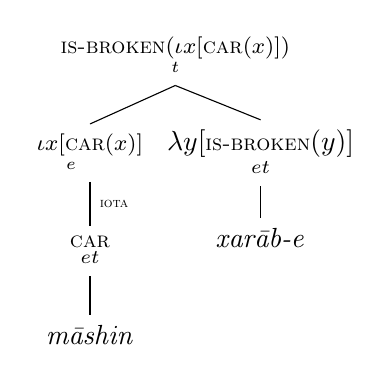
\begin{tikzpicture}[level distance=35pt]
	\Tree [.{\footnotesize$\underset{t}{\footnotesize\textsc{is-broken} (\iota x [ \textsc{car}(x)])}$}
				[.{\footnotesize $\underset{e}{\iota x [\textsc{car}}(x)]$} \edge node[auto=left] {\tiny \textsc{iota}}; [.{$\underset{et}{\footnotesize\textsc{car}}$} [.\emph{m\={a}shin} ] ] ]
        		[.{$\footnotesize \underset{et}{\lambda y [\textsc{is-broken} (y)]}$} [.\emph{xar\={a}b-e} ]
        		]
			]
	\end{tikzpicture}	
} & {\scriptsize
	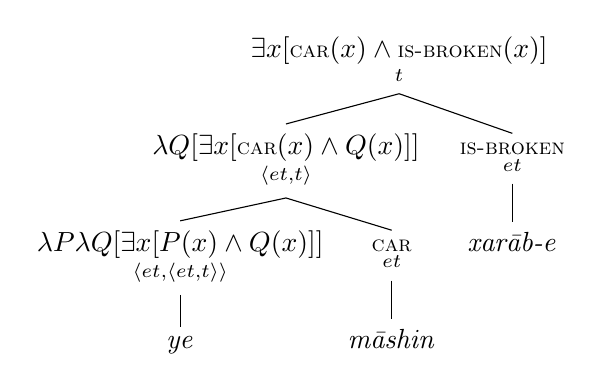
\begin{tikzpicture}[level distance=35pt]
	\Tree [.{$\underset{t}{\footnotesize \exists x [\textsc{car}(x) \land \textsc{is-broken} (x)]}$}
				[.{$\underset{\langle et,t\rangle}{\footnotesize\lambda Q [\exists x [\textsc{car}(x) \land Q (x)]]}$}
			[.{$\underset{\langle et, \langle et,t\rangle \rangle}{\footnotesize \lambda P \lambda Q [\exists x [P(x) \land Q (x)]]}$} [.\emph{ye} ] ]
    		[.{$\underset{et}{\footnotesize \textsc{car}}$} [.\emph{m\={a}shin} ] ]
    			]
        		[.{$\underset{et}{\footnotesize\textsc{is-broken}}$} [.\emph{xar\={a}b-e} ]
        		]
			]
	\end{tikzpicture}	
} \\
{\small ``The car is broken."} & {\small ``A car is broken."} \\
\end {tabular}
\caption {\small Derivations for sample definite and simple indefinite constructions in Farsi}
\label {simpletrees}
\end {figure}

\begin {figure}[h]
\centering
{\scriptsize
	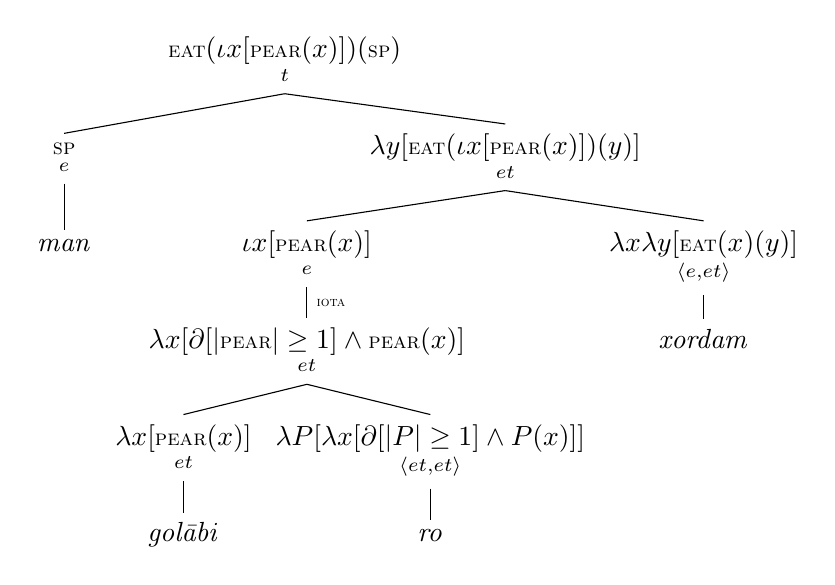
\begin{tikzpicture}[level distance=35pt]
	\Tree [.{$\underset{t}{{\footnotesize\textsc{eat}} (\iota x [{\footnotesize \textsc{pear}}(x)])({\footnotesize\textsc{sp}})}$}
				[.{$\underset{e}{{\footnotesize\textsc{sp}}}$} [.\emph{man} ] ]
        		[.{$\underset{et}{\lambda y [{\footnotesize\textsc{eat}} (\iota x [{\footnotesize \textsc{pear}}(x)])(y)]}$}
        			[.{$\underset{e}{\iota x [{\footnotesize \textsc{pear}}(x)]}$} \edge node[auto=left] {\tiny \textsc{iota}};
        			[.{$\underset{et}{\lambda x [\partial [|{\footnotesize\textsc{pear}}|\geq 1]  \land {\footnotesize \textsc{pear}} (x)]}$} 
        				[.{$\underset{et}{\lambda x [{\footnotesize\textsc{pear}} (x)]}$} [.\emph{gol\={a}bi} ] ]
        				[.{$\underset{\langle et, et \rangle}{\lambda P [\lambda x [\partial [|P|\geq 1]  \land P(x)]]}$} [.\emph{ro} ] ]
        		 	]
        		]
        			[.{$\underset{\langle e,et\rangle}{\lambda x \lambda y [{\footnotesize\textsc{eat}} (x)(y)]}$} [.\emph{xordam} ] ]
        		]
			]
	\end{tikzpicture}	
}
{\small }
\caption {\small Sample derivation of an object-marked definite in the sentence ``I ate the pear."}
\label {defra}
\end {figure}

\begin {figure}[h]
\centering
{\scriptsize
	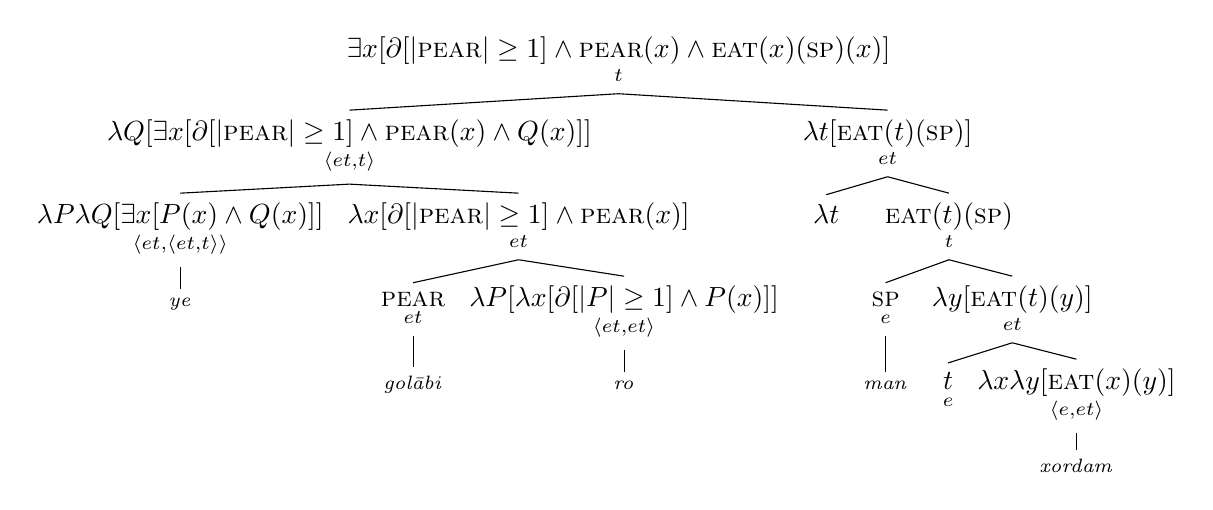
\begin{tikzpicture}[level distance=30pt]
	\Tree [.{$\underset{t}{\exists x [\partial [|\textsc{pear}|\geq 1] \land \textsc{pear}(x) \land \textsc{eat} (x)(\textsc{sp}) (x)]}$}
    		[.{$\underset{\langle et,t\rangle}{\lambda Q [\exists x [\partial [|\textsc{pear}|\geq 1] \land \textsc{pear}(x) \land Q (x)]]}$}
    			[.{$\underset{\langle et, \langle et,t\rangle \rangle}{\lambda P \lambda Q [\exists x [P(x) \land Q (x)]]}$} [.\emph{{\scriptsize ye}} ] ]
        		[.{$\underset{et}{\lambda x [\partial [|\textsc{pear}|\geq 1]  \land \textsc{pear} (x)]}$} 
        			[.{$\underset{et}{\textsc{pear}}$} [.\emph{{\scriptsize gol\={a}bi}} ] ]
        			[.{$\underset{\langle et, et \rangle}{\lambda P [\lambda x [\partial [|P|\geq 1]  \land P(x)]]}$} [.\emph{{\scriptsize ro}} ] ]
        		 ]
    		 ]
    		[.{$\underset{et}{\lambda t [\textsc{eat} (t)(\textsc{sp})]}$}
    			[.{$\lambda t$} ]
        		[.{$\underset{t}{\textsc{eat} (t)(\textsc{sp})}$}
        			[.{$\underset{e}{\textsc{sp}}$} [.\emph{{\scriptsize man}} ] ]
            		[.{$\underset{et}{\lambda y [\textsc{eat} (t)(y)]}$}
                		[.{$\underset{e}{t}$} ]
            		 	[.{$\underset{\langle e,et\rangle}{\lambda x \lambda y [\textsc{eat} (x)(y)]}$} [.\emph{{\scriptsize xordam}} ] ]
            		 ]
        		 	]
    			]
			]
	\end{tikzpicture}	
}
\caption {\small Sample derivation of an object-marked indefinite in the sentence ``I ate a certain pear/one of the pears."}
\label {indefra}
\end {figure}
\newpage
\bibliographystyle{apalike}
\bibliography{/Users/Masoud/Google/library/Bibliography.bib}

%For \cite{karimi1990obliqueness}, \emph{r\={a}} has two meaning components: 1. Uniqueness: the object-marked NP denotes a unique (specific) individual 2. Identifiability: the speaker knows the unique referent of the object-marked NP. Indefinite markers such as \emph{ye} signal whether the referent is presumed to be known by the hearer or not. \ref{KarimiTable} whether was to signal wether The difference between \emph{r\={a}}-marked definites and indefinites lied in the knowledge state of speakers and hearers. The referent of a definite NP was known to both the speaker and the hearer while the referent of an indefinite NP   was  considered uniqueness to be the main contribution of  fails to capture the distribution of the object marker. Here I show that R\={a} appears on nominals that are not epistemically specific, and epistemically specific referents can appear without R\={a}. 
%
%\begin {table}
%\begin {tabular} {l | c | c | c}
%Construction & Unique & Speaker Identifiable & Hearer Identifiable \\ \hline
%NP-\emph{ra} & + & + & + \\
%ye-NP-ra & + & + & - \\
%ye-NP & - & - & - \\
%\end {tabular}
%\caption {The semantic components of Persian definite and indefinite constructions in \cite{karimi1990obliqueness}}
%\label{KarimiTable}
%\end {table}

\end {document}